
% This LaTeX was auto-generated from MATLAB code.
% To make changes, update the MATLAB code and republish this document.

\documentclass{article}
\usepackage{graphicx}
\usepackage{color}

\sloppy
\definecolor{lightgray}{gray}{0.5}
\setlength{\parindent}{0pt}

\begin{document}

    
    
\subsection*{Contents}

\begin{itemize}
\setlength{\itemsep}{-1ex}
   \item Problem 7.27
   \item Setup
   \item Plot
\end{itemize}


\subsection*{Problem 7.27}

\begin{verbatim}
clear; close all; clc;
\end{verbatim}


\subsection*{Setup}

\begin{verbatim}
n = 15;
y = 25:35;
markov = n./y;
chebys = n./(y-n).^2;
cherno = exp(n-y).*(y./n).^n;
centlim = qfunc((y-n)./sqrt(n));
prob = cumsum(y.^(n-1).*exp(-y)/factorial(n-1));
\end{verbatim}


\subsection*{Plot}

\begin{verbatim}
figure(1)
semilogy(y,markov,y,chebys,y,cherno,y,centlim,y,prob);
legend('Markov', 'Chebyshev', 'Chernoff', 'Central Limit', 'Actual');
title('Bound Comparison in Log Space');
\end{verbatim}

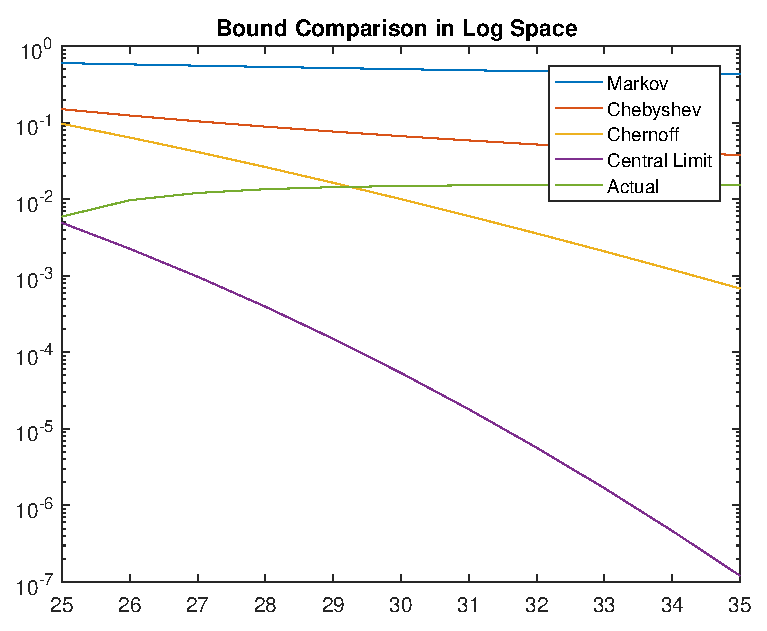
\includegraphics [width=4in]{prob7_27_01.eps}
\begin{verbatim}
figure(2)
plot(y,markov,y,chebys,y,cherno,y,centlim,y,prob);
legend('Markov', 'Chebyshev', 'Chernoff', 'Central Limit', 'Actual');
title('Bound Comparison in Linear Space');
\end{verbatim}

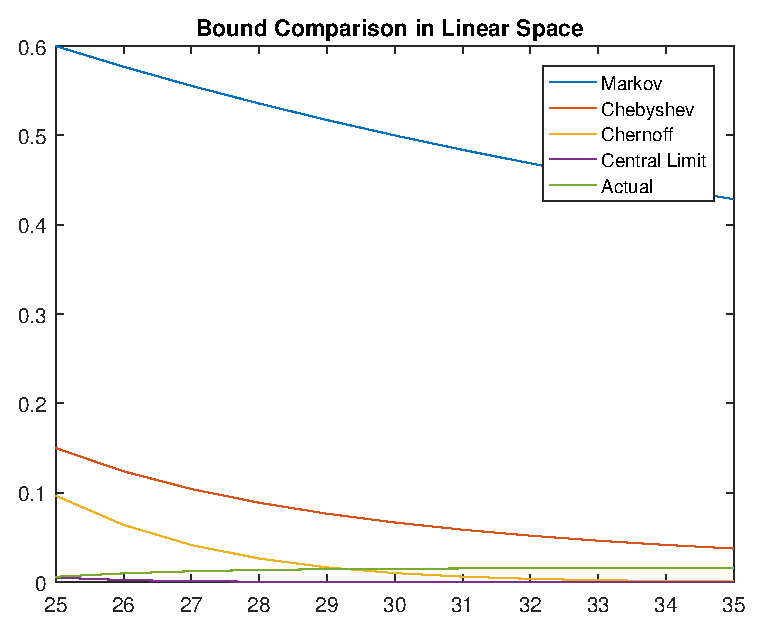
\includegraphics [width=4in]{prob7_27_02.eps}



\end{document}
    
